% !TEX root = ../discretemath.tex

\section{Классическая функция Мёбиуса. Обратная к дзете}

\subsection{ЧУМ натуральных чисел по делимости}

Рассмотрим ЧУМ $(\mathbb N,\,|\,)$: $a\le b\Leftrightarrow a\mid b$. Часть диаграммы Хассе:

\begin{center}
	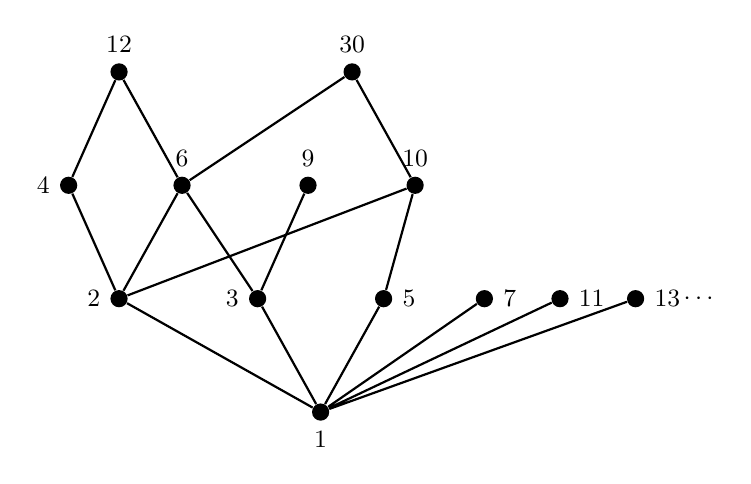
\begin{tikzpicture}[
		nd/.style   = {circle, fill=black, inner sep=2.2pt},
		lbl/.style  = {font=\small},
		every label/.style = {font=\small},
		scale = 0.8
		]
		\node[nd, label={[lbl]below:$1$}]    (n1)  at ( 0.0, 0.0) {};
		\node[nd, label={[lbl]left:$2$}]     (n2)  at (-3.2, 1.8) {};
		\node[nd, label={[lbl]left:$3$}]     (n3)  at (-1.0, 1.8) {};
		\node[nd, label={[lbl]right:$5$}]    (n5)  at ( 1.0, 1.8) {};
		\node[nd, label={[lbl]right:$7$}]    (n7)  at ( 2.6, 1.8) {};
		\node[nd, label={[lbl]right:$11$}]   (n11) at ( 3.8, 1.8) {};
		\node[nd, label={[lbl]right:$13$}]   (n13) at ( 5.0, 1.8) {};
		\node[lbl] at (6.0, 1.8) {$\cdots$};
		\node[nd, label={[lbl]left:$4$}]     (n4)  at (-4.0, 3.6) {};
		\node[nd, label={[lbl]above:$6$}]    (n6)  at (-2.2, 3.6) {};
		\node[nd, label={[lbl]above:$9$}]    (n9)  at (-0.2, 3.6) {};
		\node[nd, label={[lbl]above:$10$}]   (n10) at ( 1.5, 3.6) {};
		\node[nd, label={[lbl]above:$12$}]   (n12) at (-3.2, 5.4) {};
		\node[nd, label={[lbl]above:$30$}]   (n30) at ( 0.5, 5.4) {};
		\draw[thick] (n1)--(n2)  (n1)--(n3)  (n1)--(n5) (n1)--(n7)  (n1)--(n11) (n1)--(n13);
		\draw[thick] (n2)--(n4)  (n2)--(n6)  (n2)--(n10);
		\draw[thick] (n3)--(n6)  (n3)--(n9);
		\draw[thick] (n5)--(n10);
		\draw[thick] (n4)--(n12) (n6)--(n12);
		\draw[thick] (n6)--(n30) (n10)--(n30);
	\end{tikzpicture}
\end{center}

\begin{Definition}{Классическая функция Мёбиуса}{}
	\[
	\mu(n)=
	\begin{cases}
		0, & p^2\mid n\text{ для некоторого простого }p,\\[4pt]
		(-1)^k, & n=p_1p_2\cdots p_k\text{ — произведение $k$ различных простых.}
	\end{cases}
	\]
	В частности, $\mu(1)=1$.
\end{Definition}

\begin{Theorem}{Связь с функцией Мёбиуса ЧУМа}{}
	Для $a\mid b$ в $(\mathbb N,\,|\,)$:
	\[
	\mu_{\mathbb N}(a,b)=\mu\!\left(\tfrac{b}{a}\right).
	\]
\end{Theorem}

Это следует из изоморфизма интервалов $[a,b]\cong\bigl[1,\tfrac{b}{a}\bigr]$, откуда $\mu_{\mathbb N}(a,b)=\mu_{\mathbb N}\!\left(1,\tfrac{b}{a}\right)=:\mu\!\left(\tfrac{b}{a}\right)$.

\subsubsection*{Вычисление $\mu(1,n)$}

Для $n=p_1^{\alpha_1}\cdots p_k^{\alpha_k}$ по мультипликативности функции Мёбиуса и изоморфизму
\[
\bigl[1,\,p_1^{\alpha_1}\cdots p_k^{\alpha_k}\bigr]\cong\bigl[1,p_1^{\alpha_1}\bigr]\times\cdots\times\bigl[1,p_k^{\alpha_k}\bigr]
\]
получаем $\mu(1,n)=\mu(1,p_1^{\alpha_1})\cdots\mu(1,p_k^{\alpha_k})$. Каждый множитель — из цепочки $1<p_i<p_i^2<\cdots$:

\begin{center}
	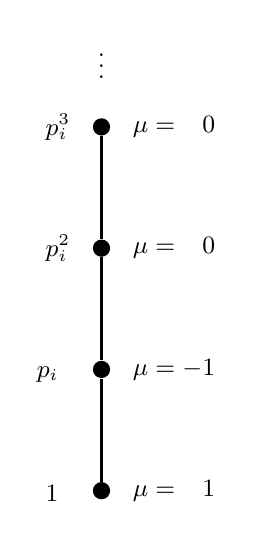
\begin{tikzpicture}[
		nd/.style  = {circle, fill=black, inner sep=2.2pt},
		lbl/.style = {font=\small},
		scale=1.1
		]
		\node[nd] (v0) at (0, 0.0) {};
		\node[nd] (v1) at (0, 1.4) {};
		\node[nd] (v2) at (0, 2.8) {};
		\node[nd] (v3) at (0, 4.2) {};
		\draw[thick] (v0)--(v1)--(v2)--(v3);
		\node[font=\small] at (0, 5.0) {$\vdots$};
		\node[lbl, anchor=east] at (-0.25, 0.0) {$1\phantom{{}^{3}}$};
		\node[lbl, anchor=east] at (-0.25, 1.4) {$p_i\phantom{{}^{3}}$};
		\node[lbl, anchor=east] at (-0.25, 2.8) {$p_i^2$};
		\node[lbl, anchor=east] at (-0.25, 4.2) {$p_i^3$};
		\node[lbl, anchor=west] at (0.25, 0.0) {$\mu = \phantom{-}1$};
		\node[lbl, anchor=west] at (0.25, 1.4) {$\mu = -1$};
		\node[lbl, anchor=west] at (0.25, 2.8) {$\mu = \phantom{-}0$};
		\node[lbl, anchor=west] at (0.25, 4.2) {$\mu = \phantom{-}0$};
	\end{tikzpicture}
\end{center}

\begin{itemize}
	\item $\mu(1,p_i)=-\mu(1,1)=-1$;
	\item $\mu(1,p_i^2)=-\mu(1,1)-\mu(1,p_i)=-1+1=0$;
	\item по индукции $\mu(1,p_i^\alpha)=0$ для всех $\alpha\ge 2$.
\end{itemize}

\begin{Corollary}{}{}
	\[
	\mu(1,n)=
	\begin{cases}
		0, & \alpha_i>1\text{ хотя бы для одного }i,\\
		(-1)^k, & \alpha_1=\cdots=\alpha_k=1.
	\end{cases}
	\]
	Это в точности классическая функция Мёбиуса $\mu(n)$.
\end{Corollary}

\subsection{Дзета-функция Римана и функция Мёбиуса}

\begin{Definition}{Дзета-функция Римана}{}
	\[
	\zeta(s)=\sum_{n=1}^{\infty}\frac{1}{n^s}=\frac{1}{1^s}+\frac{1}{2^s}+\frac{1}{3^s}+\cdots
	\]
\end{Definition}

\begin{Theorem}{Ряд Мёбиуса обратен дзете}{}
	\[
	\sum_{n=1}^{\infty}\frac{\mu(n)}{n^s}=\frac{1}{\zeta(s)}.
	\]
\end{Theorem}

\begin{proof}
	Перемножим ряды и сгруппируем по $m=nd$:
	\[
	\Bigl(\sum_{n\ge 1}\frac{\mu(n)}{n^s}\Bigr)\Bigl(\sum_{d\ge 1}\frac{1}{d^s}\Bigr)
	=\sum_{m\ge 1}\frac{1}{m^s}\sum_{n\mid m}\mu(n).
	\]
	В ЧУМ $(\mathbb N,\mid)$ условие $n\mid m$ означает $n\in[1,m]$, поэтому
	\[
	\sum_{n\mid m}\mu(n)=\sum_{1\le n\le m}\mu(1,n)=
	\begin{cases}1,&m=1,\\0,&m>1,\end{cases}
	\]
	по эквивалентной форме определения функции Мёбиуса (обнуление суммы по отрезку). Значит,
	\[
	\Bigl(\sum_{n\ge 1}\frac{\mu(n)}{n^s}\Bigr)\zeta(s)=\sum_{m\ge 1}\frac{[m=1]}{m^s}=1,
	\]
	откуда $\sum_{n\ge 1}\dfrac{\mu(n)}{n^s}=\dfrac{1}{\zeta(s)}$.
\end{proof}

\begin{Remark}{}{}
	Тождество $\sum_{n\mid m}\mu(n)=[m=1]$ — это в точности $\mu*\mathbf 1=\varepsilon$ в терминах свёртки Дирихле: функция Мёбиуса обратна тождественной единице $\mathbf 1$. Отсюда и «обратность дзете» на уровне рядов Дирихле.
\end{Remark}
